\documentclass[11pt]{article}
\usepackage[margin=1in]{geometry}
\usepackage{amsmath, amssymb}
\usepackage{hyperref}
\usepackage{enumitem}
\usepackage{tikz}
\usetikzlibrary{arrows.meta, positioning, shapes}
\usepackage{xcolor}
\usepackage{parskip}
\usepackage{natbib}
\usepackage{microtype}
\usepackage{graphicx}

\setlength{\parskip}{2pt}
\setlength{\parindent}{0pt}

\title{\textbf{Introduction to Causal Inference}\\[0.4em]
\large Stage 2: Project Research Proposal}
\author{Gil Caplan \quad Jeremy Jornet}
\date{}

\begin{document}
\maketitle

% -------------------------------------------------------
\section{Causal Question}
% -------------------------------------------------------

\begin{center}
\textbf{Does sustained daily cigarette smoking throughout pregnancy causally\\
increase the probability of infant death before age one?}
\end{center}

\textbf{Treatment Variable}
\begin{itemize}[noitemsep, topsep=2pt]
  \item \textbf{Variable names:} \texttt{CIG1\_R}, \texttt{CIG2\_R}, \texttt{CIG3\_R}
        (daily cigarette count recodes per trimester;
        values: 0\,=\,no cigarettes per day, 1\,=\,1--5/day, \ldots,
        5\,=\,$\geq$41/day, 6\,=\,unknown).
  \item \textbf{Treated group ($T=1$):} Mother smoked at least one cigarette
        per day on average in \emph{every} trimester
        (\texttt{CIG1\_R\,$\geq$\,1}, \texttt{CIG2\_R\,$\geq$\,1},
        \texttt{CIG3\_R\,$\geq$\,1}), ensuring sustained exposure
        throughout the entire pregnancy.
  \item \textbf{Control group ($T=0$):} Mother reported zero cigarettes per day
        in every trimester (\texttt{CIG1\_R\,=\,0}, \texttt{CIG2\_R\,=\,0},
        \texttt{CIG3\_R\,=\,0}).
\end{itemize}

\textbf{Outcome Variable}
\begin{itemize}[noitemsep, topsep=2pt]
  \item \textbf{Definition:} $Y=1$ if the infant died before their first birthday, $Y=0$ otherwise; derived from \texttt{FLGND} (death-linkage indicator), appended to every birth record in the NCHS denominator-plus file~\cite{nchs2015}.
\end{itemize}

\textbf{Temporal ordering.}
Smoking during pregnancy is recorded on the birth certificate before the
infant is born, while infant death can only occur after birth. Reverse
causality is therefore impossible by design.


\textbf{Primary estimand.} Using the potential outcomes framework, let $Y^{(1)}$ be the infant mortality outcome under sustained smoking and $Y^{(0)}$ the outcome under never-smoking. We target the 

\textbf{Average Treatment Effect.} $\tau = E[Y^{(1)} - Y^{(0)}]$. We additionally report the ATT from propensity score matching for comparison.

% -------------------------------------------------------
\section{Existing Knowledge and Related Literature}
% -------------------------------------------------------

The relationship between prenatal smoking and adverse infant outcomes is among the most studied topics in perinatal epidemiology. Dietz et al.~\cite{dietz2010} estimate that roughly 5--8\% of preterm births, 13--19\% of term low-birth-weight deliveries, and 5--7\% of infant deaths in the United States are attributable to prenatal smoking, placing the population-attributable fraction at roughly one in fourteen infant deaths. Cnattingius~\cite{cnattingius2004} documents that smoking prevalence during pregnancy is strongly socioeconomically patterned, which motivates our concern about confounding.

Biologically, nicotine causes uteroplacental vasoconstriction, carbon monoxide displaces fetal oxygen, and tobacco impairs placental angiogenesis, converging on hypoxia, growth restriction, preterm delivery, and abruption~\cite{cnattingius2004}. Wisborg et al.~\cite{wisborg2000} found a dose-dependent association with SIDS (adjusted OR $\approx$3.5); Salihu and Wilson~\cite{salihu2007} document heterogeneous effects by dose and mortality subtype.

Despite this large observational literature, few studies apply formal causal methods. Most adjust for birth weight which is a post-treatment mediator. Our contribution is to bring an explicit causal framework to a question
largely studied through associational methods

% -------------------------------------------------------
\section{Data}
% -------------------------------------------------------

We use the \textbf{2015 Cohort Linked Birth/Infant Death Data Set}~\cite{nchs2015},
published by the National Center for Health Statistics (NCHS), CDC. The file
follows all U.S. infants born in 2015 through their first birthday,
covering approximately 3.98 million births of which 23,357 are linked to a
death certificate (99.4\% linkage rate). Birth certificate data, recording
maternal characteristics, prenatal behaviour, and obstetric information,
are collected at delivery and submitted by states to NCHS under the Vital
Statistics Cooperative Program. When an infant dies, the corresponding death
certificate is filed and linked back to the birth record by the state of
death, yielding a single combined record per infant. The outcome $Y=1$ is
assigned to infants with a linked death record, $Y=0$ otherwise.

Key \textbf{observed pre-treatment confounders} available in the data:

\begin{center}
\small
\begin{tabular}{lll}
\hline
\textbf{Variable} & \textbf{Field} & \textbf{Role} \\
\hline
Mother's education    & \texttt{MEDUC}                    & SES proxy; predicts smoking and infant health \\
Mother's age          & \texttt{MAGER}                    & Younger mothers smoke more; age affects mortality risk \\
Race/Hispanic origin  & \texttt{MRACEHISP}                & Differential smoking prevalence and healthcare access \\
Marital status        & \texttt{DMAR}                     & Social support and economic resource proxy \\
WIC participation     & \texttt{WIC}                      & SES proxy; WIC confers nutrition and care benefits \\
Payment/insurance     & \texttt{PAY\_REC}                 & Medicaid vs.\ private insurance as SES indicator \\
Pre-pregnancy diabetes& \texttt{RF\_PDIAB}                & Pre-existing risk factor for adverse outcomes \\
Pre-pregnancy hypert. & \texttt{RF\_PHYPE}                & Pre-existing risk factor \\
Pre-pregnancy BMI     & \texttt{BMI\_R}                   & Reflects pre-existing health status before pregnancy \\
Father's education    & \texttt{FEDUC}                    & Household SES proxy correlated with maternal smoking \\
Father's age          & \texttt{FAGE11}                   & Household SES proxy correlated with maternal smoking \\
\hline
\end{tabular}
\end{center}

\vspace{1em}
\textbf{Mediators.} Birth weight (\texttt{BRTHWGT}) and gestational age
(\texttt{COMBGEST}) are \textbf{post-treatment mediators}: the literature
consistently shows that smoking causes low birth weight and prematurity,
which in turn raise infant mortality risk~\cite{dietz2010, cnattingius2004}.




% -------------------------------------------------------
\section{Causal Assumptions}
% -------------------------------------------------------

\subsection{Consistency}
We assume $Y^{(t)} = Y$ whenever $T = t$. Treatment is binary and explicitly defined; partial quitters are excluded. Consistency holds approximately because the primary biological mechanisms (nicotine-driven vasoconstriction, fetal hypoxia) are dose-dependent rather than mechanism-dependent. The dataset captures cigarettes only; other tobacco products are not recorded.

\subsection{Stable Unit Treatment Value Assumption (SUTVA)}
Interference is implausible: one mother's smoking cannot alter another infant's mortality risk. Multiple versions of treatment exist (dose, brand), but our binary definition averages over these, shifting the estimand to the ATE over the distribution of intensities among sustained smokers.

\subsection{Conditional ignorability.} We assume that, conditional on the
observed covariates, treatment assignment is independent of the potential
outcomes. The dataset is rich for a population-level study,
covering socioeconomic status, maternal health history, and demographics,
and several variables, education, insurance, WIC participation, serve
as partial proxies for harder-to-measure constructs. Nevertheless, the
literature consistently highlights maternal mental health, psychological
stress, alcohol consumption, and substance use as predictors of both
smoking persistence and adverse infant outcomes~\cite{cnattingius2004,
richmond2017}, none of which are recorded in birth certificate data.
To the extent these unobserved factors are positively associated with
both treatment and outcome, our estimates should be interpreted as upper
bounds on the true causal effect.

\subsection{Positivity}
After applying all reporting-flag and confounder-completeness filters, the analytic sample contains 2,938,232 records: 174,225 sustained smokers (5.9\%) and 2,764,007 never-smokers (94.1\%). We modelled $e(\mathbf{X})=P(T=1\mid\mathbf{X})$ via logistic regression on all eleven confounders. The estimated PS spans $[0.0003,\,0.654]$ among treated and $[0.0002,\,0.671]$ among controls, yielding a common support region of $[0.0003,\,0.654]$ --- positivity holds nominally across the full treated PS range (Appendix, Figures~\ref{fig:ps_hist}--\ref{fig:ps_logit}). However, a large share of controls pile up near PS\,$\approx$\,0 (high-education, high-income never-smokers for whom sustained smoking is nearly impossible), reflecting \emph{practical} positivity violations in those strata. Trimming at the 1st/99th percentiles of the treated PS removes 8.5\% of the sample and is applied as a pre-specified sensitivity check; more aggressive 5th/95th trimming (removing 32.5\%) is also evaluated.

% -------------------------------------------------------
\section{Pearl's Causal Graph}
% -------------------------------------------------------

Figure~\ref{fig:dag} presents the proposed DAG. Observed confounders affect both the probability of sustained smoking and infant mortality independently. Alcohol/substance use is an important unobserved confounder not captured in the data. Birth weight and gestational age lie on the causal path (mediators) and are excluded from adjustment to estimate the \emph{total} effect.

\begin{figure}[ht]
\centering
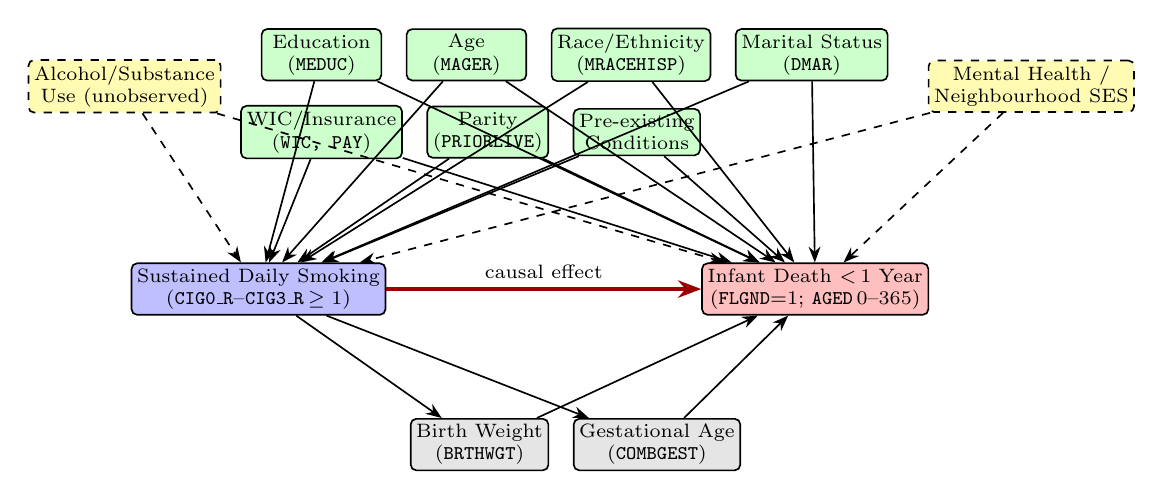
\begin{tikzpicture}[
  node distance=0.3cm,
  every node/.style={font=\scriptsize, align=center},
  obs/.style    ={rectangle, draw, fill=green!20,  rounded corners=2pt, minimum width=1.52cm, minimum height=0.50cm, inner sep=2pt},
  unobs/.style  ={rectangle, draw, fill=yellow!30, rounded corners=2pt, minimum width=1.45cm, minimum height=0.50cm, inner sep=2pt, dashed},
  treat/.style  ={rectangle, draw, fill=blue!25,   rounded corners=2pt, minimum width=2.1cm,  minimum height=0.62cm, inner sep=2pt},
  outc/.style   ={rectangle, draw, fill=red!25,    rounded corners=2pt, minimum width=2.1cm,  minimum height=0.62cm, inner sep=2pt},
  med/.style    ={rectangle, draw, fill=gray!20,   rounded corners=2pt, minimum width=1.45cm, minimum height=0.50cm, inner sep=2pt},
  ->, >=Stealth, semithick
]

%% Treatment and Outcome (Y anchored right of T -- guarantees identical height)
\node[treat] (T)
  {Sustained Daily Smoking\\(\texttt{CIG0\_R}--\texttt{CIG3\_R}$\,\geq1$)};
\node[outc, right=4.0cm of T] (Y)
  {Infant Death ${<}$\,1 Year\\(\texttt{FLGND}=1; \texttt{AGED}\,0--365)};

%% Row 1: 4 observed confounders (above the T-Y axis)
\node[obs, above=2.3cm of T, xshift=0.8cm]  (edu)  {Education\\(\texttt{MEDUC})};
\node[obs, right=0.3cm of edu]  (age)  {Age\\(\texttt{MAGER})};
\node[obs, right=0.3cm of age]  (race) {Race/Ethnicity\\(\texttt{MRACEHISP})};
\node[obs, right=0.3cm of race] (mar)  {Marital Status\\(\texttt{DMAR})};

%% Row 2: 3 observed confounders (below row 1)
\node[obs, below=0.3cm of edu]  (ses)  {WIC/Insurance\\(\texttt{WIC, PAY})};
\node[obs, right=0.3cm of ses]  (par)  {Parity\\(\texttt{PRIORLIVE})};
\node[obs, right=0.3cm of par]  (hlth) {Pre-existing\\Conditions};

%% Unobserved confounders: placed LEFT of edu and RIGHT of mar
%% (completely outside the confounder block's x-range -- no overlap possible)
\node[unobs, left=0.5cm of edu, yshift=-0.4cm] (alc)
  {Alcohol/Substance\\Use (unobserved)};
\node[unobs, right=0.5cm of mar, yshift=-0.4cm] (mh)
  {Mental Health /\\Neighbourhood SES};

%% Mediators (below T, between T and Y)
\node[med, below right=1.3cm and 0.3cm of T] (bw) {Birth Weight\\(\texttt{BRTHWGT})};
\node[med, right=0.3cm of bw]                (ga) {Gestational Age\\(\texttt{COMBGEST})};

%% Causal arrow
\draw[red!60!black, very thick] (T) -- (Y)
  node[midway, above, font=\scriptsize, black]{causal effect};

%% Observed confounders → T and → Y
\foreach \c in {edu,age,race,mar,ses,par,hlth}{
  \draw (\c) -- (T);
  \draw (\c) -- (Y);
}

%% Unobserved → T and → Y
\draw[dashed] (alc) -- (T);
\draw[dashed] (alc) -- (Y);
\draw[dashed] (mh)  -- (T);
\draw[dashed] (mh)  -- (Y);

%% Mediator paths
\draw (T) -- (bw);  \draw (bw) -- (Y);
\draw (T) -- (ga);  \draw (ga) -- (Y);

\end{tikzpicture}

\smallskip
\noindent\footnotesize
\tikz\node[rectangle,draw,fill=green!20,rounded corners=2pt,inner sep=2pt,font=\scriptsize]{Observed Confounder};~
\tikz\node[rectangle,draw,fill=yellow!30,dashed,rounded corners=2pt,inner sep=2pt,font=\scriptsize]{Unobserved Confounder};~
\tikz\node[rectangle,draw,fill=blue!25,rounded corners=2pt,inner sep=2pt,font=\scriptsize]{Treatment};~
\tikz\node[rectangle,draw,fill=red!25,rounded corners=2pt,inner sep=2pt,font=\scriptsize]{Outcome (Y)};~
\tikz\node[rectangle,draw,fill=gray!20,rounded corners=2pt,inner sep=2pt,font=\scriptsize]{Mediator (not adjusted)};

\caption{Proposed DAG for the causal effect of sustained daily prenatal smoking on infant mortality. All observed pre-treatment confounders (including marital status and parity) constitute the adjustment set. Alcohol/substance use is highlighted as the most important unobserved confounder absent from the data. Birth weight and gestational age are post-treatment mediators excluded from adjustment to estimate the total effect.}
\label{fig:dag}
\end{figure}

% -------------------------------------------------------
\section{Anticipated Challenges}
% -------------------------------------------------------

\begin{itemize}[noitemsep, topsep=2pt, leftmargin=*]
  \item \textbf{Alcohol and substance use: key unobserved confounder.} Alcohol/drug use is strongly correlated with sustained smoking and independently causes infant mortality (FASD, SIDS, abruption), yet is absent from the dataset. This is the primary upward bias threat; we address it via E-value analysis (see \S\ref{sec:sensitivity}).

  \item \textbf{Self-reported smoking and misclassification.} Smoking is self-reported on the birth certificate; social desirability bias leads some smokers to under-report, attenuating the estimated effect toward the null. We use pre-pregnancy smoking (\texttt{CIG0\_R}) as a partial validation anchor: a mother reporting no in-pregnancy smoking despite non-zero pre-pregnancy counts is a probable misclassifier.

  \item \textbf{Incomplete reporting area and missing data.} Tobacco fields require \texttt{F\_TOBACCO\,=\,1}; pre-existing condition checkboxes (\texttt{RF\_PDIAB}, \texttt{RF\_PHYPE}) require their own reporting flags, available only in revised-certificate states. These restrictions reduce the analytic sample. Several confounders carry unknown codes (\texttt{MEDUC\,=\,9}, \texttt{PAY\_REC\,=\,9}); a missing data sensitivity check is planned.

  \item \textbf{Rare outcome and treatment imbalance.} The infant mortality rate is $\approx$\,5.9 per 1,000 live births, and sustained smokers comprise approximately 4--6\% of the analytic sample. Together these produce sparse treated-and-died cells and potentially extreme inverse-probability weights. We will use stabilised weights and bootstrap all confidence intervals (1,000 replications).

  \item \textbf{Mediator exclusion and total vs.\ direct effects.} Excluding birth weight and gestational age from the adjustment set means we estimate the \emph{total} causal effect, including pathways through fetal growth restriction and prematurity. We will state this explicitly and not interpret results as reflecting only direct nicotine effects on infant mortality.

\end{itemize}

% -------------------------------------------------------
\section{Planned Estimation Methods}
% -------------------------------------------------------

We adopt a multi-method strategy to assess robustness to modelling assumptions, since conditional ignorability cannot be verified from the data. All methods target the ATE; the ATT from propensity score matching is reported as a secondary estimate.

\textbf{Outcome regression (S-Learner).} Logistic regression of $Y$ on $T$ and all confounders provides a stable, interpretable ATE baseline.

\textbf{T-Learner.} Separate logistic models are fitted for $T=1$ and $T=0$; potential outcomes are imputed for all units and averaged into the ATE. This allows the covariate-outcome relationship to differ across arms.

\textbf{Propensity Score Matching (ATT).} We estimate $e(\mathbf{X}) = P(T=1 \mid \mathbf{X})$ via logistic regression and match each sustained smoker to the most similar never-smoker on the logit of the propensity score (nearest-neighbour, with caliper $= 0.2 \times$\,SD of the logit). This estimates the ATT -- reported as a secondary, policy-relevant quantity.

\textbf{Inverse Probability Weighting (IPW).} Observations are reweighted by stabilised IPW weights to construct a pseudo-population with balanced covariates; the ATE is estimated as a weighted outcome difference.

\textbf{Augmented IPW / Doubly Robust (AIPW).}~\cite{robins1994} Combines the outcome model with the propensity model; consistent if either is correctly specified. This is our \textbf{primary ATE estimator}. All confidence intervals are via non-parametric bootstrap (1,000 replications).

% -------------------------------------------------------
\section{Planned Sensitivity Checks}
\label{sec:sensitivity}
% -------------------------------------------------------

\begin{enumerate}[noitemsep, topsep=2pt, leftmargin=*]
  \item \textbf{E-value for unobserved confounding.}~\cite{vanderweele2017} For the primary AIPW estimate, we compute the E-value: the minimum strength of association (on the risk ratio scale) that an unobserved confounder would need with both treatment and outcome to fully explain away the observed effect. An E-value smaller than the known association between alcohol use and infant mortality would indicate the result is not robust to this confounder.

  \item \textbf{Treatment threshold.} Re-estimate with $T=1$ defined as $\geq$5 cigarettes/day (\texttt{CIG1\_R\,$\geq$\,2}) and $\geq$10/day (\texttt{CIG1\_R\,$\geq$\,3}) in all trimesters. Monotonic dose-response strengthens causal interpretation.

  \item \textbf{``Throughout'' operationalisation.} Re-estimate requiring only the three trimesters (dropping the pre-pregnancy \texttt{CIG0\_R} requirement) and requiring only 2 of 3 trimesters. Stability across these definitions assesses robustness to the operationalisation of ``throughout.''

  \item \textbf{Missing data.} Compare complete-case analysis to results under multiple imputation (predictive mean matching, 20 imputations) for confounders with unknown codes.

  \item \textbf{Propensity score trimming.} Re-estimate IPW and AIPW after trimming at the 1st/99th and 5th/95th propensity percentiles to assess reliance on poorly-supported strata.

  \item \textbf{Singleton restriction.} Restrict to \texttt{DPLURAL\,=\,1}. Multiple births carry structurally higher mortality risk and lower maternal smoking prevalence, potentially confounding estimates.

\end{enumerate}


\newpage
% -------------------------------------------------------
\bibliographystyle{plain}
{\small
\begin{thebibliography}{9}

\bibitem{dietz2010}
Dietz, P.M., England, L.J., Shapiro-Mendoza, C.K., Tong, V.T., Farr, S.L., \& Callaghan, W.M. (2010).
Infant morbidity and mortality attributable to prenatal smoking in the US.
\textit{American Journal of Preventive Medicine}, 39(1), 45--52.

\bibitem{cnattingius2004}
Cnattingius, S. (2004).
The epidemiology of smoking during pregnancy: smoking prevalence, maternal characteristics, and pregnancy outcomes.
\textit{Nicotine \& Tobacco Research}, 6(Suppl\,2), S125--S140.

\bibitem{wisborg2000}
Wisborg, K., Kesmodel, U., Henriksen, T.B., Olsen, S.F., \& Secher, N.J. (2000).
Exposure to tobacco smoke in utero and the risk of stillbirth and death in the first year of life.
\textit{American Journal of Epidemiology}, 154(4), 322--327.

\bibitem{salihu2007}
Salihu, H.M., \& Wilson, R.E. (2007).
Epidemiology of prenatal smoking and perinatal outcomes.
\textit{Early Human Development}, 83(11), 713--720.

\bibitem{robins1994}
Robins, J.M., Rotnitzky, A., \& Zhao, L.P. (1994).
Estimation of regression coefficients when some regressors are not always observed.
\textit{Journal of the American Statistical Association}, 89(427), 846--866.

\bibitem{vanderweele2017}
VanderWeele, T.J., \& Ding, P. (2017).
Sensitivity analysis in observational research: introducing the E-value.
\textit{Annals of Internal Medicine}, 167(4), 268--274.

\bibitem{nchs2015}
National Center for Health Statistics. (2018).
\textit{2015 Cohort Linked Birth/Infant Death Data Set: Public Use Data File Documentation}.
Centers for Disease Control and Prevention.


\bibitem{richmond2017}
Richmond, R.C., et al. (2017).
Maternal smoking in pregnancy and offspring depression: a cross cohort
and negative control study.
\textit{Scientific Reports}, 7, 12579.

\bibitem{yuan2023}
Yuan, S., et al. (2023).
Dose--response association between maternal smoking during pregnancy
and the risk of infant death: a nationwide, population-based,
retrospective cohort study.
\textit{eClinicalMedicine}, 57, 101835.


\end{thebibliography}
}

% -------------------------------------------------------
\appendix
\section{Propensity Score Overlap Diagnostics}
\label{sec:appendix_ps}
% -------------------------------------------------------

The following figures are produced by fitting a logistic regression of $T$ on all eleven observed confounders (Table~1) using the analytic sample of 2,938,232 records. Figures are used to visually assess the overlap (positivity) assumption discussed in \S4.4.

\begin{figure}[ht]
\centering

\includegraphics[width=0.92\textwidth]{ps_overlap_histogram.png}
\caption{Mirror histogram of estimated propensity scores $\hat{e}(\mathbf{X})$ by treatment arm. Treated units (blue, above axis) are compared with control units (orange, below axis), both normalised to proportions. The shaded green region marks the common support $[0.0003,\,0.654]$; dashed lines indicate the 5th and 95th percentiles of the treated PS ($0.012$ and $0.420$) used for the trimming sensitivity check.}
\label{fig:ps_hist}
\end{figure}

\begin{figure}[ht]
\centering

\includegraphics[width=0.92\textwidth]{ps_overlap_logit.png}
\caption{Kernel density estimates of the logit propensity score $\text{logit}\,\hat{e}(\mathbf{X})$ by treatment arm. The treated distribution (blue) peaks at logit\,$\approx -1.3$ and the control distribution (orange) at logit\,$\approx -4.2$. The shaded overlap region represents strata where both treated and control units exist and causal comparisons are well-supported.}
\label{fig:ps_logit}
\end{figure}

\end{document}
